% =====================================================================
% Snippet: embedded-graph.tex
% =====================================================================
% USAGE: Small graph visualization (5-7 nodes + edges) for embedding
% inside a stage. Examples: molecule structure, social network,
% neural connectivity, citation graph.
%
% Two variants:
%   A. Star pattern (1 center + N neighbors) — GAT neighbor sampling
%   B. Cycle pattern (N nodes in a ring) — molecule structure
%
% Copy %% COPY-START / END (pick A or B), replace:
%   - nodes: number / positions
%   - colors: node fill colors
%   - origin_x, origin_y, radius
% =====================================================================

\documentclass[tikz,border=10pt]{standalone}
\usepackage{xcolor,tikz}
\usetikzlibrary{positioning,calc}

\definecolor{acaBlueLine}{HTML}{3060A8}
\definecolor{acaBlueFill}{HTML}{6890C8}
\definecolor{acaTealLine}{HTML}{1F8F8F}
\definecolor{acaTealFill}{HTML}{5AB8B8}
\definecolor{acaPurpleLine}{HTML}{6E3FA0}
\definecolor{acaPurpleFill}{HTML}{A878D0}
\definecolor{acaGreenLine}{HTML}{389050}
\definecolor{acaGreenFill}{HTML}{6CB088}
\definecolor{acaOrangeLine}{HTML}{D06020}
\definecolor{acaOrangeFill}{HTML}{F08850}
\definecolor{acaGreyLine}{HTML}{606060}

\tikzset{
  graph node/.style={
    circle, draw=acaBlueLine, fill=white,
    line width=0.7pt, minimum size=0.55cm,
    font=\scriptsize, inner sep=0pt,
  },
  center node/.style={
    circle, draw=acaPurpleLine, fill=acaPurpleFill,
    line width=1.0pt, minimum size=0.7cm,
    font=\scriptsize\bfseries, text=white, inner sep=0pt,
  },
  graph edge/.style={
    line width=0.6pt, color=acaGreyLine,
  },
  attn edge/.style={
    line width=#1, color=acaPurpleLine,    % thickness encodes weight
  },
}

\begin{document}
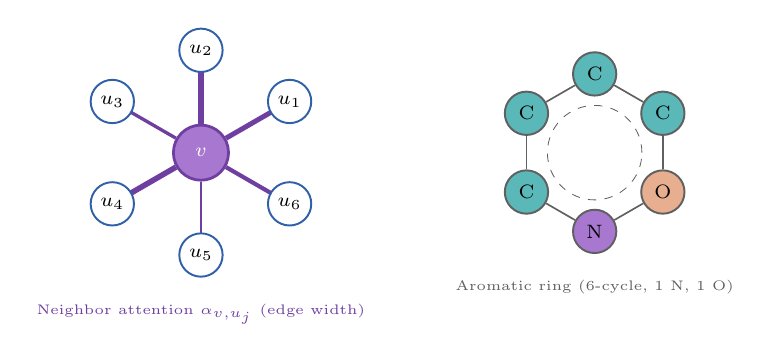
\begin{tikzpicture}

%% COPY-START (Variant A: GAT-style star with attention weights) =====

\def\xO{0}
\def\yO{0}
\def\rad{1.3}

% Center node
\node[center node] (v) at (\xO, \yO) {$v$};

% 6 neighbors at angles 0/60/120/180/240/300
% Edge thickness encodes attention weight α_v,j (just visual)
\foreach \i/\ang/\w in {1/30/1.8pt, 2/90/2.5pt, 3/150/1.2pt,
                       4/210/2.0pt, 5/270/0.8pt, 6/330/1.5pt} {
  \pgfmathsetmacro\nx{\xO + \rad * cos(\ang)}
  \pgfmathsetmacro\ny{\yO + \rad * sin(\ang)}
  \draw[attn edge=\w] (v) -- (\nx, \ny);
  \node[graph node] (u\i) at (\nx, \ny) {$u_\i$};
}
% Label
\node[font=\tiny, color=acaPurpleLine, anchor=north]
  at (\xO, \yO - \rad - 0.5)
  {Neighbor attention $\alpha_{v,u_j}$ (edge width)};

%% COPY-END Variant A ================================================


%% COPY-START (Variant B: Molecule cycle structure) ==================

\def\xC{5}
\def\yC{0}
\def\radC{1.0}

% 6 atoms in cycle (benzene-like)
\foreach \i/\ang/\atom/\col in {
  1/30/C/acaTealFill, 2/90/C/acaTealFill,
  3/150/C/acaTealFill, 4/210/C/acaTealFill,
  5/270/N/acaPurpleFill, 6/330/O/acaOrangeLine!50
} {
  \pgfmathsetmacro\ax{\xC + \radC * cos(\ang)}
  \pgfmathsetmacro\ay{\yC + \radC * sin(\ang)}
  \node[graph node, fill=\col, draw=acaGreyLine] (a\i) at (\ax, \ay) {\atom};
}
% Bonds (cycle: 1-2-3-4-5-6-1, with alternating double-bonds visual)
\foreach \a/\b in {1/2, 2/3, 3/4, 4/5, 5/6, 6/1} {
  \draw[graph edge] (a\a) -- (a\b);
}
% Aromatic ring inner circle (optional, decoration)
\draw[acaGreyLine, dashed, line width=0.3pt]
  (\xC, \yC) circle (\radC * 0.6);
% Label
\node[font=\tiny, color=acaGreyLine, anchor=north]
  at (\xC, \yC - \radC - 0.5)
  {Aromatic ring (6-cycle, 1 N, 1 O)};

%% COPY-END Variant B ================================================

\end{tikzpicture}
\end{document}
